\documentclass[dvipsnames]{article}
\usepackage{pgfplots}
\usetikzlibrary{decorations.markings}
\pgfplotsset{compat=newest}

% \def\Point{36.9}

\begin{document}

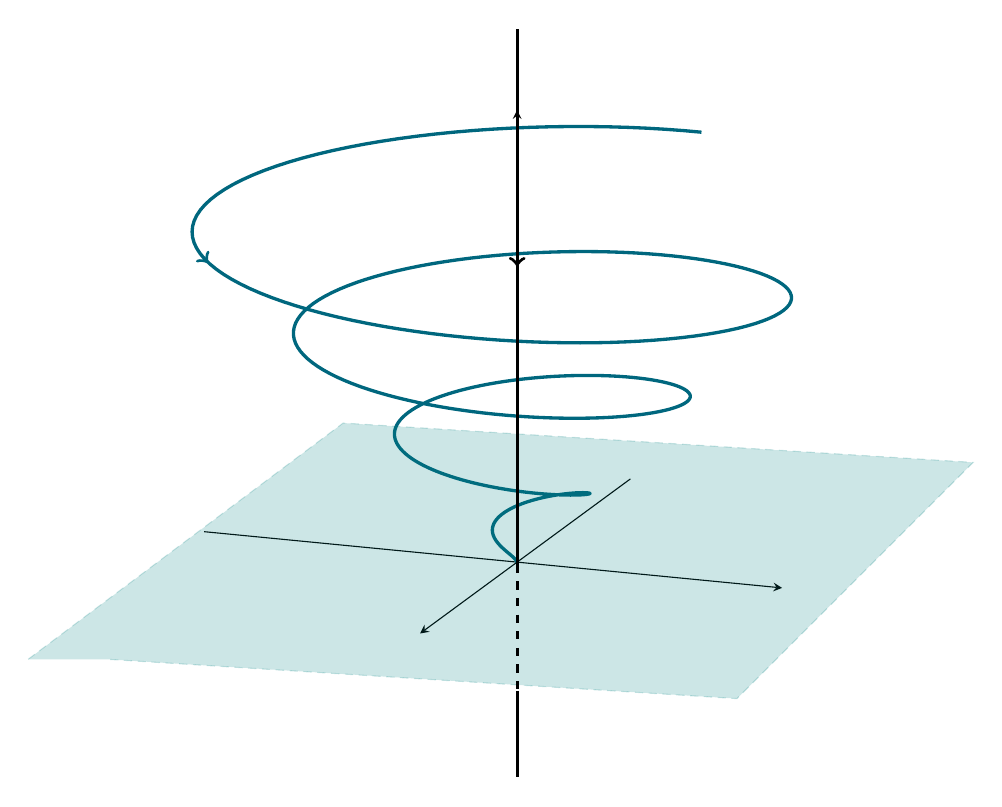
\begin{tikzpicture}
  \begin{axis}[
    view={-20}{-20}, %угол обзора
    axis lines=middle,
    zmax=60,
    height=10cm,
    xtick=\empty,
    ytick=\empty,
    ztick=\empty
    ]
    \addplot3+[,ytick=\empty,yticklabel=\empty,
    mark=none,
    very thick,
    color={rgb,255:red,0; green,103; blue,126},
    domain=0:15*pi,
    postaction={decorate,
                decoration={markings,mark=at position 0.8 with {\arrow{<}}}
               },
    samples=400,
    samples y=0,
    ]
    (-{x*sin(0.15*pi*deg(x))},{x*cos(0.15*pi*deg(x)},{x});
  \end{axis}
  \draw[teal,densely dashed][fill = teal, opacity=0.2]  (-1,0) -- (3,3) -- (11,2.5) -- (8,-0.5) -- (0,0);
  \draw[very thick] [->] (5.21,5) --(5.21,4.99);
  \draw[very thick] (5.21,8) --(5.21,1.2);
  \draw[very thick, dashed] (5.21,1.2) --(5.21,-0.4);
  \draw[very thick] (5.21,-0.4) --(5.21,-1.5);
\end{tikzpicture}

\end{document}